\documentclass[10pt]{article}
\usepackage[margin=0.85in]{geometry}
\usepackage{graphicx,booktabs,amsmath,xcolor,listings}
\usepackage[colorlinks=true,linkcolor=blue,urlcolor=blue]{hyperref}
\graphicspath{{../figs/}}
\lstset{basicstyle=\ttfamily\footnotesize,frame=single,backgroundcolor=\color{black!4}}
\setlength{\parskip}{2pt}
\pagestyle{empty}
\newcommand{\nt}{\texttt{n\_threads}}
\newcommand{\nd}{\texorpdfstring{\texttt{nd}}{nd}}

\begin{document}
% \begin{center}{\large\bfseries Performance of the multi-RHS dielectric BIE solver}\end{center}

\title{Performance of the multi-RHS dielectric BIE solver}

\maketitle

\noindent

I benchmarked the performance of the FMM3D more detailedly on the $96$ core genoa nodes, with \texttt{OMP\_NUM\_THREADS} \emph{and} \texttt{OPENBLAS\_NUM\_THREADS} pinned. 
The major takeaways are listed below:
\begin{itemize}
   \item[1.] For highly non-uniform distributions (e.g. slab with edge refinement, see Fig.~\ref{f:interface}), the FMM3D can only reach maximum throughput of about $2.4 M$ eval/s, which is about $7\times$ slower than the uniform distribution under the same settings.
   \item[2.] For non-uniform distributions, the speedup from threads saturates at about $30\times$, and the speedup from batching $\nd$ saturates at about $2.5\times$ with $\nd=36$.. Combined they reach about $76\times$ maximum speedup.
   \item[3.] The previous almost linear speedup from $\nd$ was an artifact of thread contamination.
\end{itemize}

\begin{figure}[htbp]
   \centering
   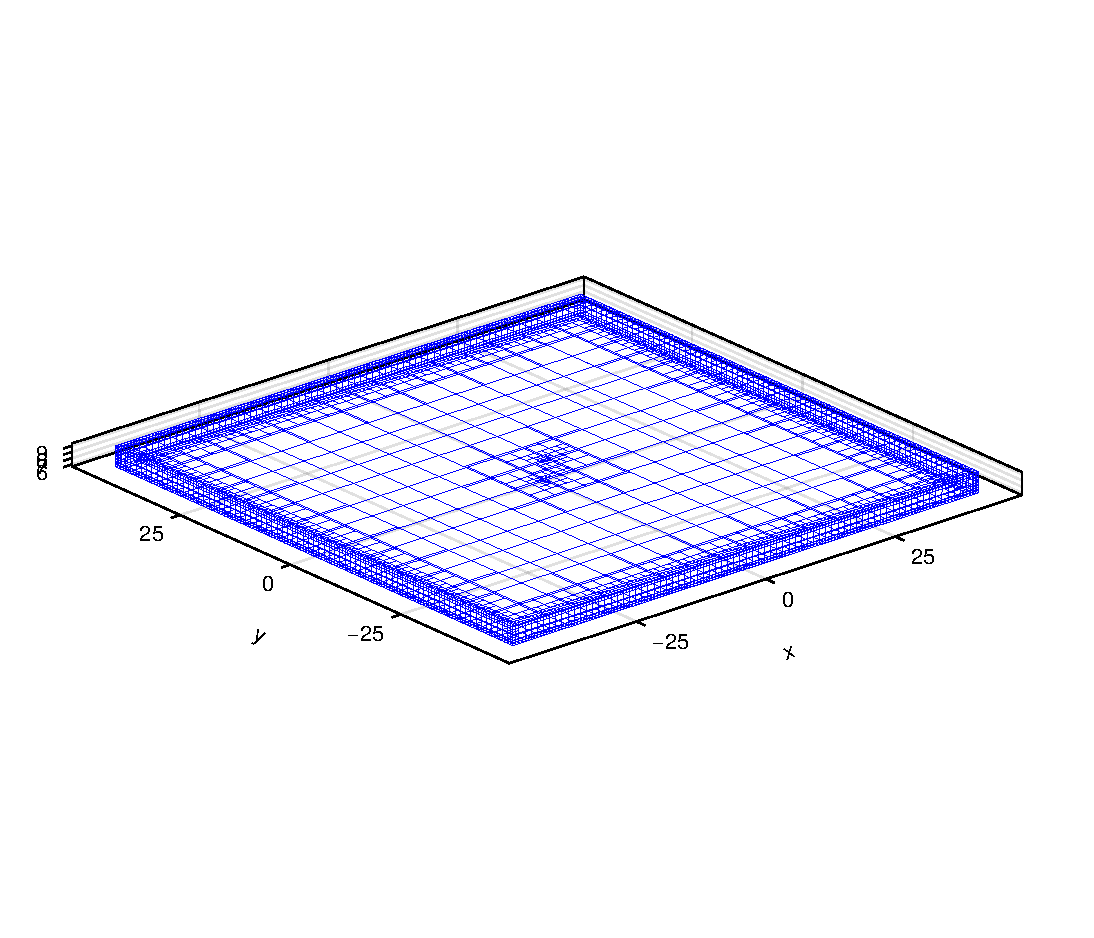
\includegraphics[width=0.6\textwidth]{interface.pdf}
   \caption{The slab interface geometry used for benchmarking (non-uniform).}
   \label{f:interface}
\end{figure}

\section{Uniform vs.\ non-uniform distributions}

The same FMM kernel was run on the real slab interface (Fig.~\ref{f:interface}) and on a 3D-uniform cloud of equal $N$. 
The slab is at most \textbf{$7\times$ slower} than the uniform case: peak throughput $2.37M$ (slab) vs $12.87M$ (uniform), and uniform dominates along every knob (Fig.~\ref{f:tput}). The penalty (Table~\ref{t:pen}) grows with thread count and factors at $N{=}461\,376$ as
$$
\underbrace{7.03\times}_{\text{96 thr}}=\underbrace{2.75\times}_{\text{1 thr (extra work)}}\times
\underbrace{2.54\times}_{\text{scaling gap}},
$$
where the first factor is the extra work from the slab's non-uniform geometry (e.g.\ heavier near field and deeper tree structure), and
the scaling gap because the slab parallelizes $1\!\to\!96$ by only $20.4\times$ vs the uniform
$52.0\times$.

\begin{table}[htbp]\centering\footnotesize
\caption{Slab/uniform ratio of $t_{\mathrm{fmm}}$, $\nd{=}36$ (times the slab is slower).}\label{t:pen}
\begin{tabular}{@{}rcccc@{}}\toprule
threads & $N{=}33\,696$ & $N{=}93\,312$ & $N{=}215\,136$ & $N{=}461\,376$\\\midrule
1  & $2.61 \times$ & $1.04 \times$ & $1.99 \times$ & $2.75 \times$\\
32 & $3.56 \times$ & $1.35 \times$ & $4.23 \times$ & $5.09 \times$\\
96 & $3.42 \times$ & $1.79 \times$ & $5.27 \times$ & $\textbf{7.03} \times$ \\ \bottomrule
\end{tabular}
\end{table}

\begin{figure}[htbp]\centering
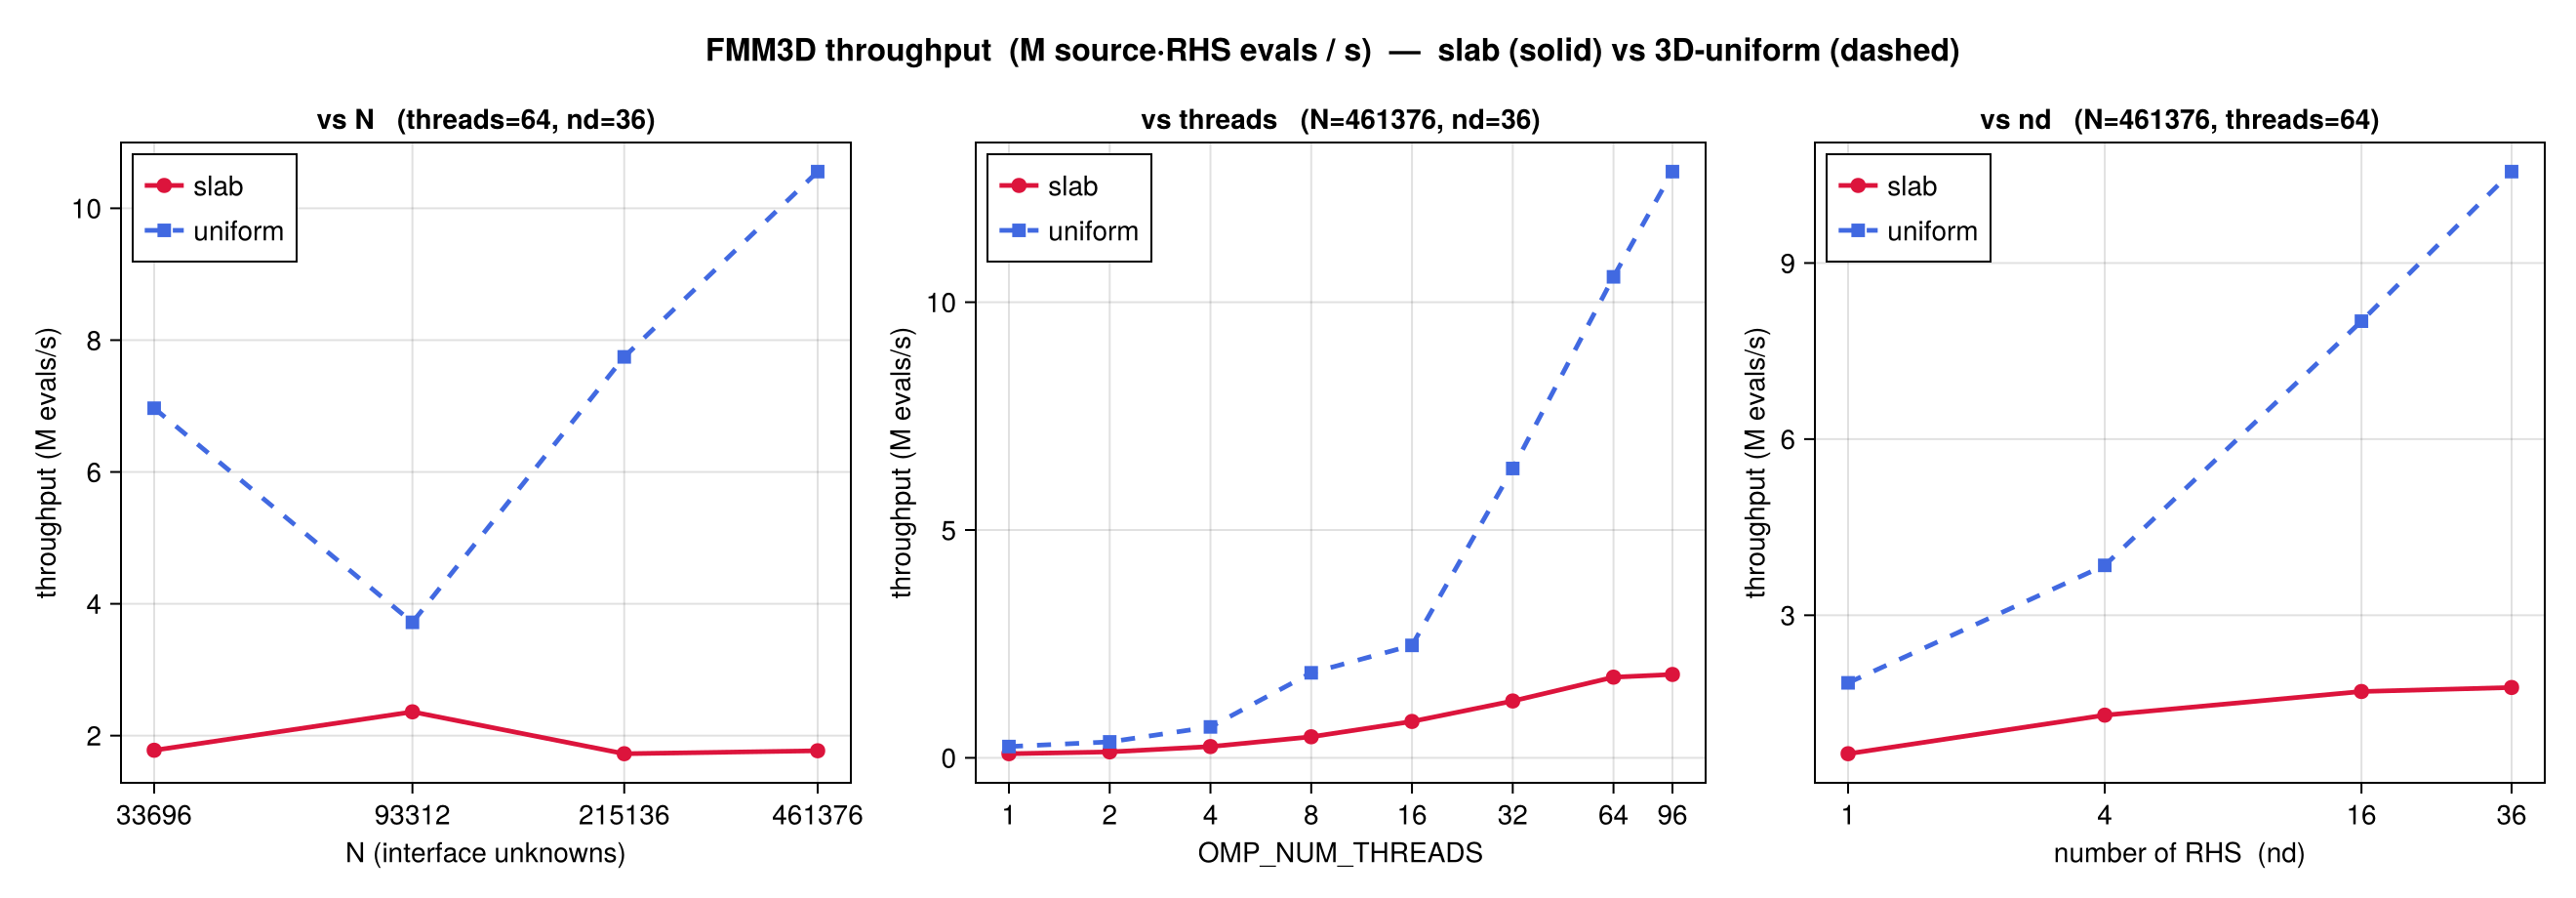
\includegraphics[width=0.97\textwidth]{fmm_throughput.png}
\caption{FMM throughput vs.\ $N$, threads, and \nd{} (slab solid red, uniform dashed blue), each
panel varying one knob (others fixed at 64 threads, $\nd{=}36$, $N{=}461\,376$). Uniform dominates
in every panel.}\label{f:tput}
\end{figure}


\section{Speedup from threads and \nd}

Fig.~\ref{f:bench} shows the speedup of the FMM kernel, where I fixed $N{=}461\,376$.
The results are shown in Fig.~\ref{f:bench}.
For fixed number of threads, the speedup from batching $\nd$ is from~$2.5\times$ to~$3.7\times$, and for fixed $\nd$, the speedup from threads is from~$20\times$ to~$30\times$.
The peak combined speedup from both is about $76\times$ at $\nd=36$ and 96 threads.

% Threads and \nd{} are orthogonal levers on the FMM kernel (slab, $N{=}461\,376$, from
% \texttt{fmm\_bench.csv}; Fig.~\ref{f:bench}).
% \emph{Batching \nd} amortizes a flat $\sim$3.7$\times$ that plateaus (per-RHS $t_{\mathrm{fmm}}/\nd$:
% $19.10\to7.94\to5.47\to5.14$\,s for $\nd{=}1,4,16,36$ $\Rightarrow$ $1.0,2.4,3.5,\mathbf{3.7}\times$).
% \emph{Threads} give $1\!\to\!96$ speedups of $17.9\times$ ($N{=}33$k) to $20.4\times$
% ($N{=}461$k), near-ideal to $\sim$16 threads then saturating---\textbf{96 threads $\approx$ 64}.
% Combined (Table~\ref{t:comb}) they reach $\sim$73$\times$ at $\nd{=}36$/64 threads. These are
% distinct: $\sim$3.7$\times$ (\nd), $\sim$18--20$\times$ (threads), $\sim$73$\times$ (both)---not to
% be conflated.

% \begin{table}[ht]\centering\footnotesize
% \caption{Combined per-RHS FMM speedup vs.\ $(\nd{=}1,1\,\text{thr})$, slab, $N{=}461\,376$.}\label{t:comb}
% \begin{tabular}{@{}rccccc@{}}\toprule
% threads & 1 & 8 & 16 & 64 & 96\\\midrule
% speedup & $3.7\times$ & $19\times$ & $33\times$ & $\mathbf{73\times}$ & $76\times$\\\bottomrule
% \end{tabular}
% \end{table}

\begin{figure}[ht]\centering
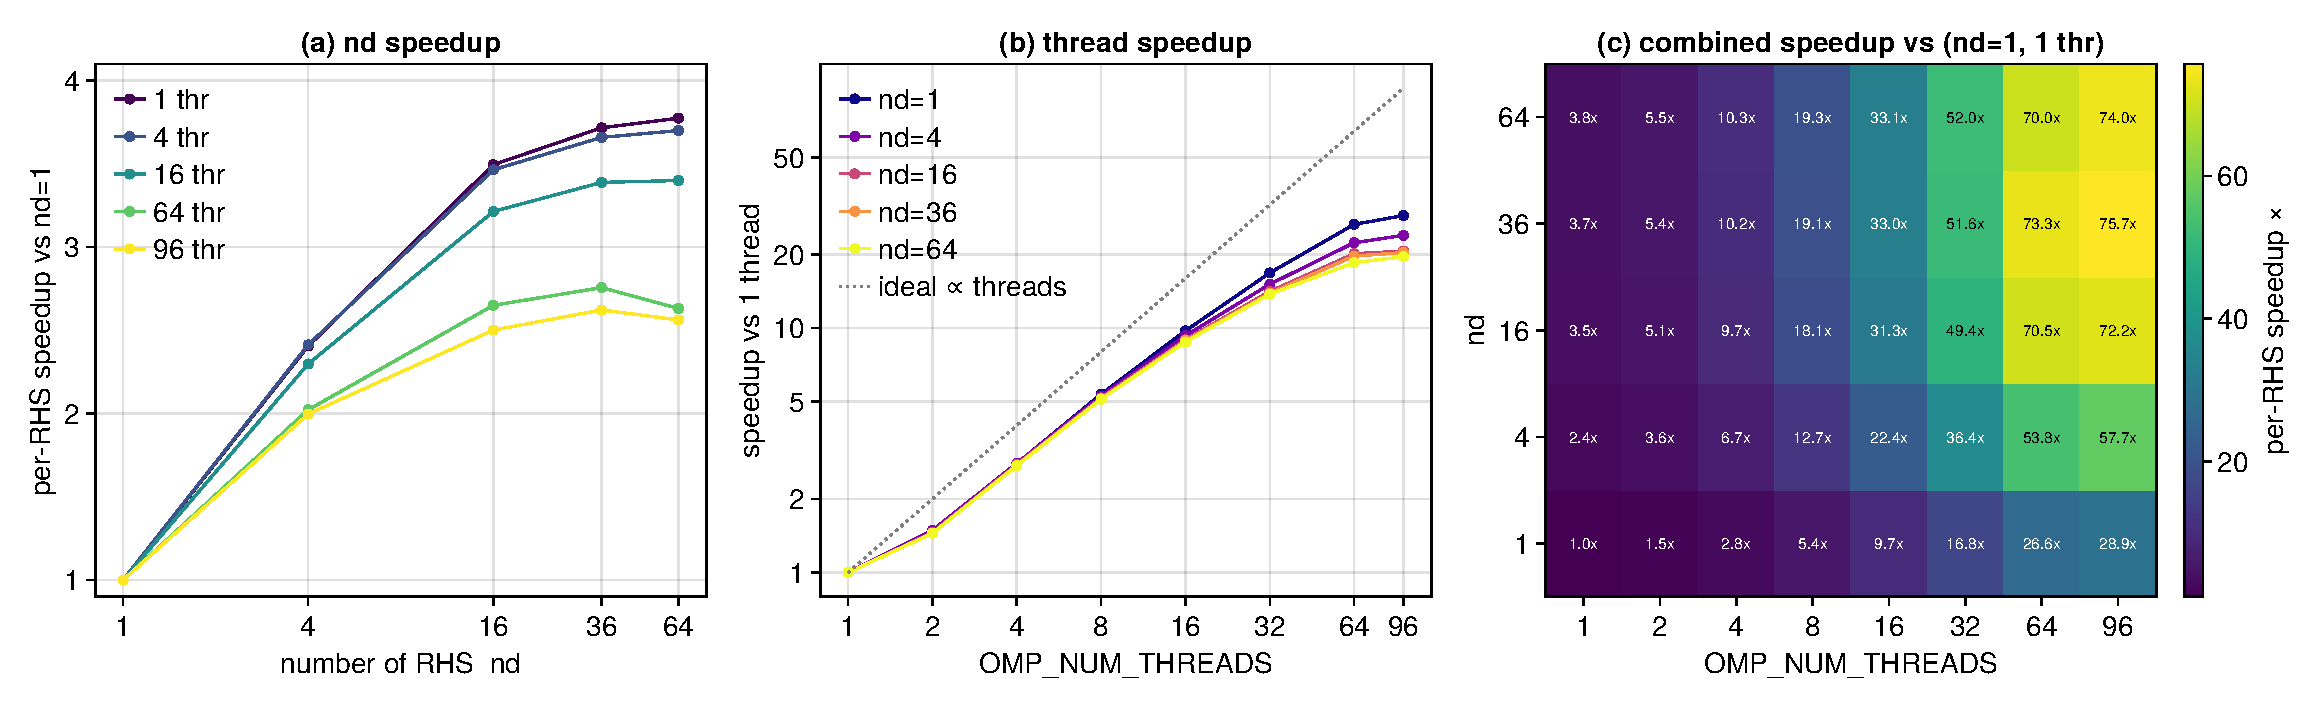
\includegraphics[width=0.95\textwidth]{fmm_speedup_grid.pdf}
\caption{Speedup of the slab FMM kernel at $N{=}461\,376$. \textbf{(a)} per-RHS \nd{} amortization
$\mathrm{nd}\cdot t(\mathrm{nd}{=}1,T)/t(\mathrm{nd},T)$ vs \nd{}, one curve per thread count $T$
(each relative to its own $\nd{=}1$; saturates $\sim$3.7$\times$ at 1 thread, lower at high $T$).
\textbf{(b)} thread speedup $t(1\,\text{thr},\mathrm{nd})/t(T,\mathrm{nd})$ vs threads, one curve per
\nd{} (saturates $\sim$20$\times$, below the ideal diagonal). \textbf{(c)} combined per-RHS speedup
$\mathrm{nd}\cdot t(1,1)/t(\mathrm{nd},T)$ over \nd$\times$threads, peaking $\sim$76$\times$.}\label{f:bench}
\end{figure}


\section{How FMM3D accelerates the multi-RHS (\nd) evaluation}
The $\nd$ density vectors are evaluated in a \emph{single} \texttt{lfmm3d} call. The point is that
the expensive, geometry-dependent quantities depend only on the source/target/box \emph{positions},
not on the charges $q$ --- so FMM3D forms each \emph{once} and reuses it across all $\nd$ densities,
with an inner \texttt{do idim=1,nd} loop doing only cheap multiply--accumulates.

\emph{Near field.} The kernel $1/r$ (the square root and reciprocal) and its gradient factor $-1/r^3$
are computed once per source--target pair, then applied to all $\nd$ charges (\texttt{l3ddirectcg}):
\begin{lstlisting}
cd = inv4pi/sqrt(dd)      ! 1/r : the expensive sqrt+divide, ONCE per source-target pair
do idim = 1,nd            ! every density reuses cd -- only multiply-adds
   pot(idim,i) = pot(idim,i) + cd*charge(idim,j) ; ...
enddo
\end{lstlisting}

\emph{Far field.} Likewise the associated-Legendre / spherical-harmonic polynomial recurrences
(\texttt{ylgndr*}, used to form and evaluate the multipole and local expansions) and the M2L
translation operators depend only on box geometry and expansion order: computed once per box and
reused inside a \texttt{do idim=1,nd} loop over the $\nd$ coefficient sets.

A direct phase breakdown (Table~\ref{t:phase}, $N{=}200$k, 1 thread)
confirms this: $\sim$\textbf{84\%} of a call is shared geometry/operator work (M2L $+$ the $1/r$ P2P
dominate), tree construction only $\sim$2\%. Only the $\sim$16\% charge-dependent arithmetic scales
with $\nd$, so $\nd{=}36$ costs $6.8\times$ (not $36\times$) one call --- giving the per-RHS ceiling
$(a{+}b)/b\approx4\times$ for the slab ($\sim$6$\times$ uniform).

\begin{table}[h]\centering\footnotesize
\caption{FMM phase times (s); $a{+}b\,\nd$ split. Tree+setup is $\sim$2\%.}\label{t:phase}
\begin{tabular}{@{}lrrrr@{}}\toprule
phase & $\nd{=}1$ & $\nd{=}36$ & $a$ & $b$\\\midrule
P2M & 0.18 & 0.83 & 0.16 & 0.019\\
M2M & 0.18 & 2.17 & 0.12 & 0.057\\
\textbf{M2L} & \textbf{2.04} & \textbf{15.94} & \textbf{1.64} & \textbf{0.40}\\
L2L & 0.17 & 2.08 & 0.11 & 0.055\\
L2P & 0.21 & 0.62 & 0.20 & 0.012\\
\textbf{P2P} & \textbf{1.13} & \textbf{4.95} & \textbf{1.02} & \textbf{0.11}\\
tree+setup & \textbf{0.09} & 0.44 & --- & ---\\\midrule
total & 3.99 & 27.04 & 3.34\,(84\%) & 0.65\\\bottomrule
\end{tabular}
\end{table}

\end{document}
